\def\mytitle{MATRICES USING PYTHON}
\def\myauthor{VAMSI SUNKARI}
\def\contact{vamsisunkari9849@gmail.com}
\def\mymodule{Future Wireless Communication (FWC)}
\documentclass[10pt, a4paper]{article}
\usepackage[a4paper,outer=1.5cm,inner=1.5cm,top=1.75cm,bottom=1.5cm]{geometry}
\twocolumn
\usepackage{graphicx}
\graphicspath{{./images/}}
\usepackage[colorlinks,linkcolor={black},citecolor={blue!80!black},urlcolor={blue!80!black}]{hyperref}
\usepackage[parfill]{parskip}
\usepackage{lmodern}
\usepackage{tikz}
 \usepackage{physics}
\usepackage{karnaugh-map}
\usepackage{setspace}
\doublespacing
%\documentclass{article}
\usepackage{tabularx}
%\usepackage{circuitikz}
\usetikzlibrary{calc}
\usepackage{amsmath}
\usepackage{amssymb}
\renewcommand*\familydefault{\sfdefault}
%\usepackage{watermark}
\usepackage{lipsum}
\usepackage{xcolor}
\usepackage{listings}
\usepackage{float}
\usepackage{titlesec}
\providecommand{\mtx}[1]{\mathbf{#1}}
\titlespacing{\subsection}{1pt}{\parskip}{3pt}
\titlespacing{\subsubsection}{0pt}{\parskip}{-\parskip}
\titlespacing{\paragraph}{0pt}{\parskip}{\parskip}
\newcommand{\figuremacro}[5]{
    \begin{figure}[#1]
        \centering
        \includegraphics[width=#5\columnwidth]{#2}
        \caption[#3]{\textbf{#3}#4}
        \label{fig:#2}
    \end{figure}
}
\newcommand{\myvec}[1]{\ensuremath{\begin{pmatrix}#1\end{pmatrix}}}
\let\vec\mathbf
\lstset{
frame=single, 
breaklines=true,
columns=fullflexible
}
\title{\mytitle}
\author{\myauthor\hspace{1em}\\\contact\\FWC22040\hspace{6.5em}IITH\hspace{0.5em}\mymodule\hspace{6em}ASSIGN-5}
\date{}
\begin{document}
 \maketitle
 \tableofcontents
\section{Construction}                                                                    \begin{center}
  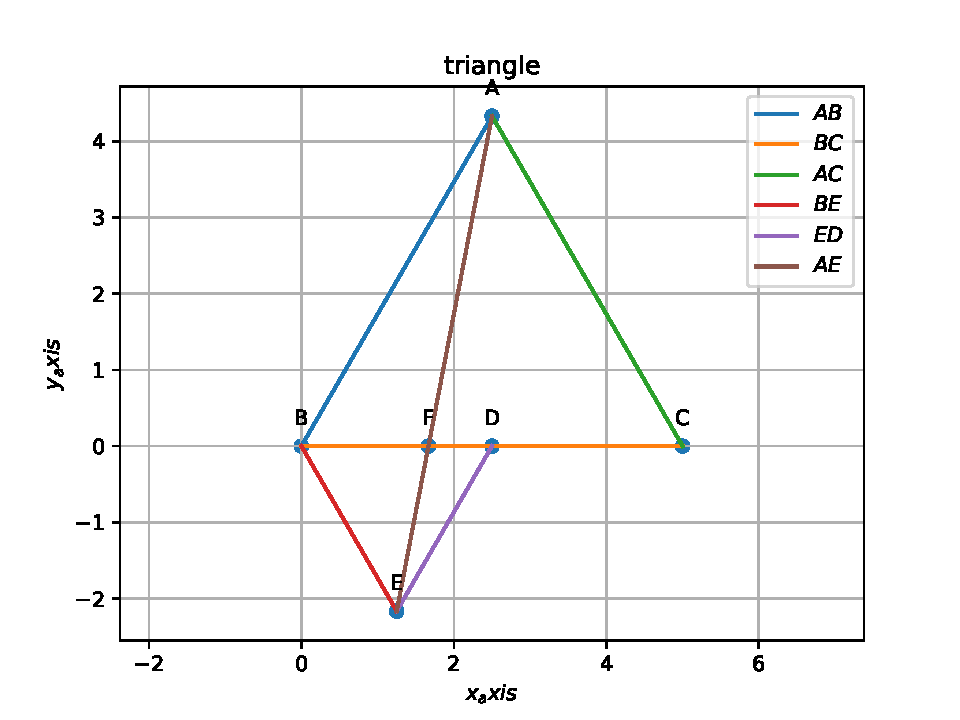
\includegraphics[scale=0.39]{par.pdf}
\\  Figure of construction
   \end{center}
   \section{Problem}
  ABC and BDE are two equilateral
triangles such that D is the mid-point of BC. If AE
intersects BC at F, show that\\
(i) ar(BDE) =1/4 ar(ABC)\\
(ii)ar(BDE) =1/2 ar(BAE)\\
(iii)ar(ABC) =2 ar(BEC)\\
(iv)ar(BFE) = ar(AFD)\\
(v)ar(BFE) =2ar(FED)\\
(vi)ar(FED) =1/8 ar(AFC)

   %  \includegraphics[scale=1.0]{diag_1.png}
   \section{Solution}
   \textbf{Theory:}\\
   \textbf{To Prove:} ar(BDE)=1/4 ar(ABC) \\
   ABC and BDE are two equilateral triangles such that D is the mid-point of BC.If AE intersets BC at F


\textbf{termux commands :}
\begin{lstlisting}
python3 matrix.py
\end{lstlisting}


The input parameters for this construction are 
\begin{center}
\begin{tabular}{|c|c|c|}
 \hline
 \textbf{Symbol}&\textbf{Value}&\textbf{Description}\\
 \hline
 r&5&AB\\
 \hline

 $\vec{A}$&$r\myvec{\cos\theta \\ \sin\theta}$%
 &Point A\\
 \hline
 $\vec{B}$&$\myvec{0 \\ 0}$%
 &Point B\\
 \hline
 $\vec{C}$&$\myvec{r \\ 0}$%
 &Point C\\
 \hline
 ${\theta}$& $\pi/3$&$ \angle $ABC\\ 
 \hline
\end{tabular}
\end{center}
\
\\
\begin{center}
$\vec{F}$ is Point of intersection of the lines BD and AE
\\
The line equation of BD is 
\begin{equation}
    \myvec{0&1}x = 0
\end{equation}
The line equation of AE is
\begin{equation}
    \myvec{-3\tan{\theta}&1}x = 2r\sin{\theta}
\end{equation}
The augmented matrix is\\ 
    $\myvec{-3\tan{\theta}&1&-2r\sin{\theta} \\ 0&1&0=}
    \xleftarrow[]{R_1 \leftarrow R_1 - R_2}
    \myvec{	    1 & 0  & \frac{2}{3}r\cos{\theta}
			    \\
			    0 & 1 & 0}$\\
   $\vec{F} = \myvec{\frac{2}{3}r\cos{\theta}\\0}$
   \ 
   \\
   \ 
   \\
   $\vec{D} = \frac{\vec{B+C}}{2}$\\
   \
\\
	$\vec{E} = {\frac{\vec{A}}{2}} \myvec{1& 0\\0& -1}=\myvec{\frac{r}{2}\cos{\theta}\\ \frac{-r}{2}\sin{\theta}}$
\\

\end{center}
\textbf{To Prove:} ar(BDE)=1/4 ar(ABC)
  \begin{center}
 
 $\vec{v1}=\vec{A-B}$\\
 $\vec{v2}=\vec{A-C}$\\
	  \begin{equation}
ar(\Delta ABC) =\frac{1}{2}\norm{\vec{v1}\times\vec{v2}}
	  \end{equation}
$\vec{v3}=\vec{B-D}$\\
 $\vec{v4}=\vec{B-E}$\\
	  \begin{equation}
 ar(\Delta BDE) =\frac{1}{2}\norm{\vec{v3}\times\vec{v4}}
          \end{equation}
  $ar(BDE)= \frac{1}{4} ar(ABC)$

 \end{center}
 \textbf{To Prove:}  ar(BDE)=1/2 ar(BAE) 
 \begin{center}
$\vec{v5}=\vec{A-E}$\\
$\vec{v6}=\vec{A-B}$\\
	 \begin{equation}
 ar(\Delta BAE) =\frac{1}{2}\norm{\vec{v5}\times\vec{v6}}
	 \end{equation}
 $ar(BDE)=\frac{1}{2} ar(BAE)$
\end{center}
 \textbf{To Prove:}  ar(ABC)=2 ar(BEC) 
 \begin{center}
 $\vec{v7}=\vec{B-C}$\\
$\vec{v8}=\vec{B-E}$\\
	 \begin{equation}
 ar(\Delta BEC) =\frac{1}{2}\norm{\vec{v7}\times\vec{v8}}
	 \end{equation}
 $ar(ABC)=2 ar(BEC)$
 \end{center}
 \textbf{To Prove:}  ar(BFE)=ar(AFD) 
 \begin{center}
 $\vec{v9}=\vec{B-F}$\\
$\vec{v10}=\vec{B-E}$\\
$\vec{v11}=\vec{A-D}$\\
$\vec{v12}=\vec{A-F}$\\
	 \begin{equation}
 ar(\Delta BFE) =\frac{1}{2}\norm{\vec{v9}\times\vec{v10}}
	 \end{equation}
	 \begin{equation}
 ar(\Delta AFD) =\frac{1}{2}\norm{\vec{v11}\times\vec{v12}}
	 \end{equation}

 ar(BFE)=ar(AFD)
 \end{center}
 \textbf{To prove} : ar(BFE) =2ar(FED)
\begin{center}
$\vec{v13}=\vec{F-E}$\\
$\vec{v14}=\vec{F-D}$\\
	\begin{equation}
 ar(\Delta FED) =\frac{1}{2}\norm{\vec{v13}\times\vec{v14}}
	\end{equation}
 $ar(BFE) =2ar(FED)$   
\end{center}
\textbf{To prove} : $ar(FED) =\frac{1}{8} ar(AFC)$
\begin{center}
$\vec{v15}=\vec{A-F}$\\
$\vec{v16}=\vec{A-C}$\\
	\begin{equation}
ar(\Delta AFC) =\frac{1}{2}\norm{\vec{v15}\times\vec{v16}}
	\end{equation}
 $ar(FED) =\frac{1}{8} ar(AFC)$   
\end{center}
The below python code realizes the above construction: 
\begin{lstlisting}
https://github.com/Vamsi9849/iithfwc/blob/main/Matrix_line/codes/matrix.py
\end{lstlisting}   
\bibliographystyle{ieeetr}
\end{document}
